\documentclass{article}
\usepackage[utf8]{inputenc}

\title{Procesamiento De Grafos}
\author{Saúl Montes De Oca Martínez}
\date{30 de Octubre de 2019}

\usepackage{natbib}
\usepackage{graphicx}
\usepackage{listings}
\usepackage{bm}
\lstset{frame=tb,
  language=Java,
  aboveskip=3mm,
  belowskip=3mm,
  showstringspaces=false,
  columns=flexible,
  basicstyle={\small\ttfamily},
  numbers=none,
  numberstyle=\tiny\color{gray},
  keywordstyle=\color{blue},
  commentstyle=\color{dkgreen},
  stringstyle=\color{mauve},
  breaklines=true,
  breakatwhitespace=true,
  tabsize=3
}
\newcommand{\uvec}[1]{\boldsymbol{\hat{\textbf{#1}}}}


\begin{document}
\twocolumn
\maketitle
\begin{abstract}
  El siguiente documento tiene como propósito demostrar al lector la importación de un dataset y el manejo del mismo utilizando la herramienta Gephi para su análisis.
\end{abstract}
\section{Introducción}
Los grafos son un conjunto de puntos llamados vertices los cuales tiene la característica de contar con una unión por líneas llamadas aristas (que pueden contar con un peso) representado como G = (V, E). Pueden ser de dos tipos, dirigidos y no dirigidos.
Para la implementación de la programación siguiente se uso el lenguaje C++ y se instaló la librería de SNAP (Stanford Network Analysis Project) para su uso en particular.

\begin{figure}[h!]
\centering
\includegraphics[scale=1]{dirigido.gif}
\caption{Grafo Dirigido}
\label{fig:dirigido}
\end{figure}

\section{Importación de dataset de SNAP}
El dataset elejido para la importación del mismo fue el de Facebook encontrado en la página de SNAP en la sección de SNAP Datasets, dentro de Social Network como ego-Facebook. Concecuentemente se descargó el archivo .txt que contiene el grafo y se crearon los códigos basados de un repositorio de Github.

\section{Implementación}
Para la implementación se uso como fuente un repositorio de github (mostrado como fuente en el mismo código) y de ahí se editaron los códigos que se podrán observar en la última sección del documento. Una vez obtenido los archivos exportados a sus formatos se empleo el uso de la herramienta Gephi explicada a continuación.

\section{Gephi}
Para el uso de Gephi se uso como muestra el archivo GraphML exportado del dataset, obtenido por los códigos. De este archivo en específico se obtuvo una gráfica usando dicho software, se exploro por la herramienta y se obtuvieron estos resultados de entre muchos.

\begin{center}
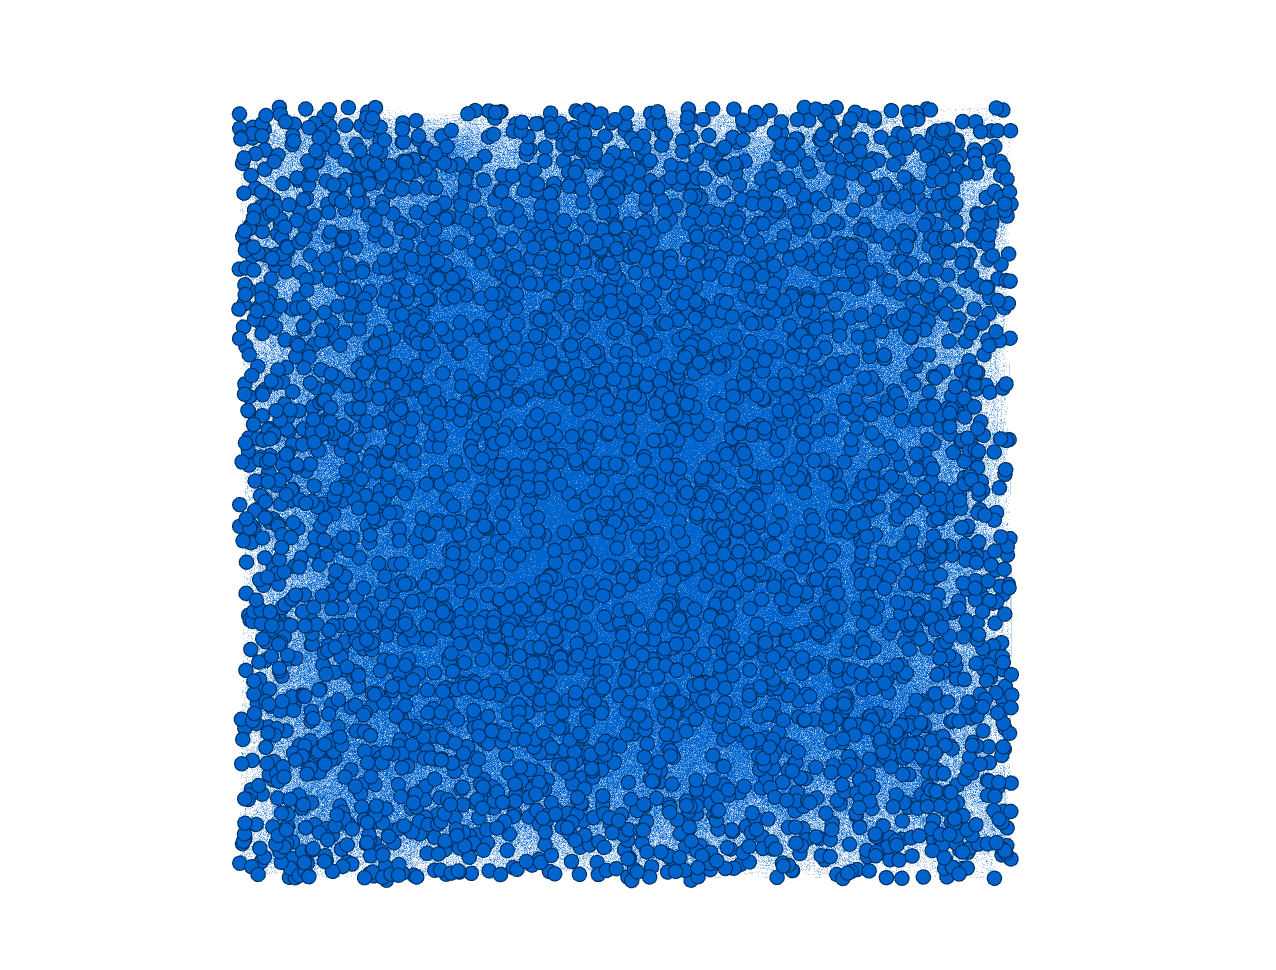
\includegraphics[scale=.2]{Grafo.png}
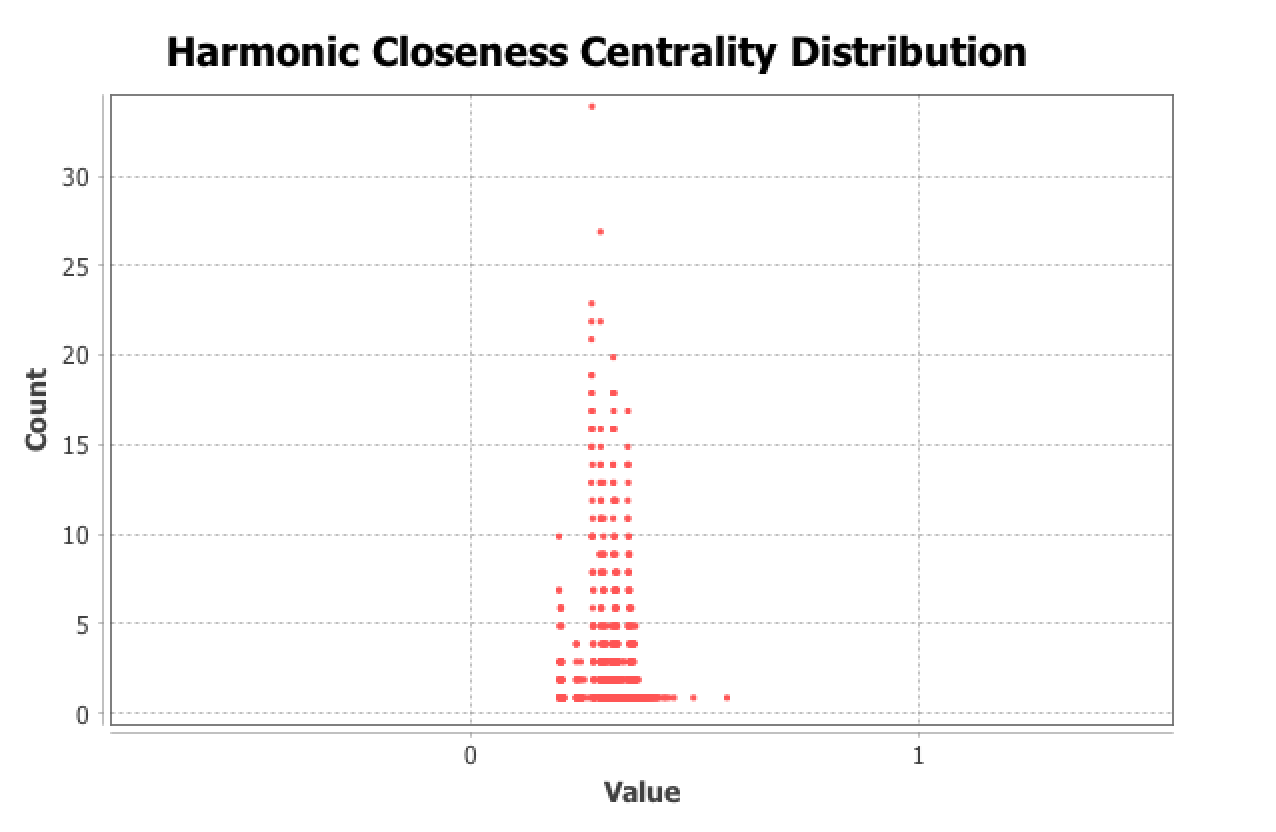
\includegraphics[scale=.2]{HCCD.png}
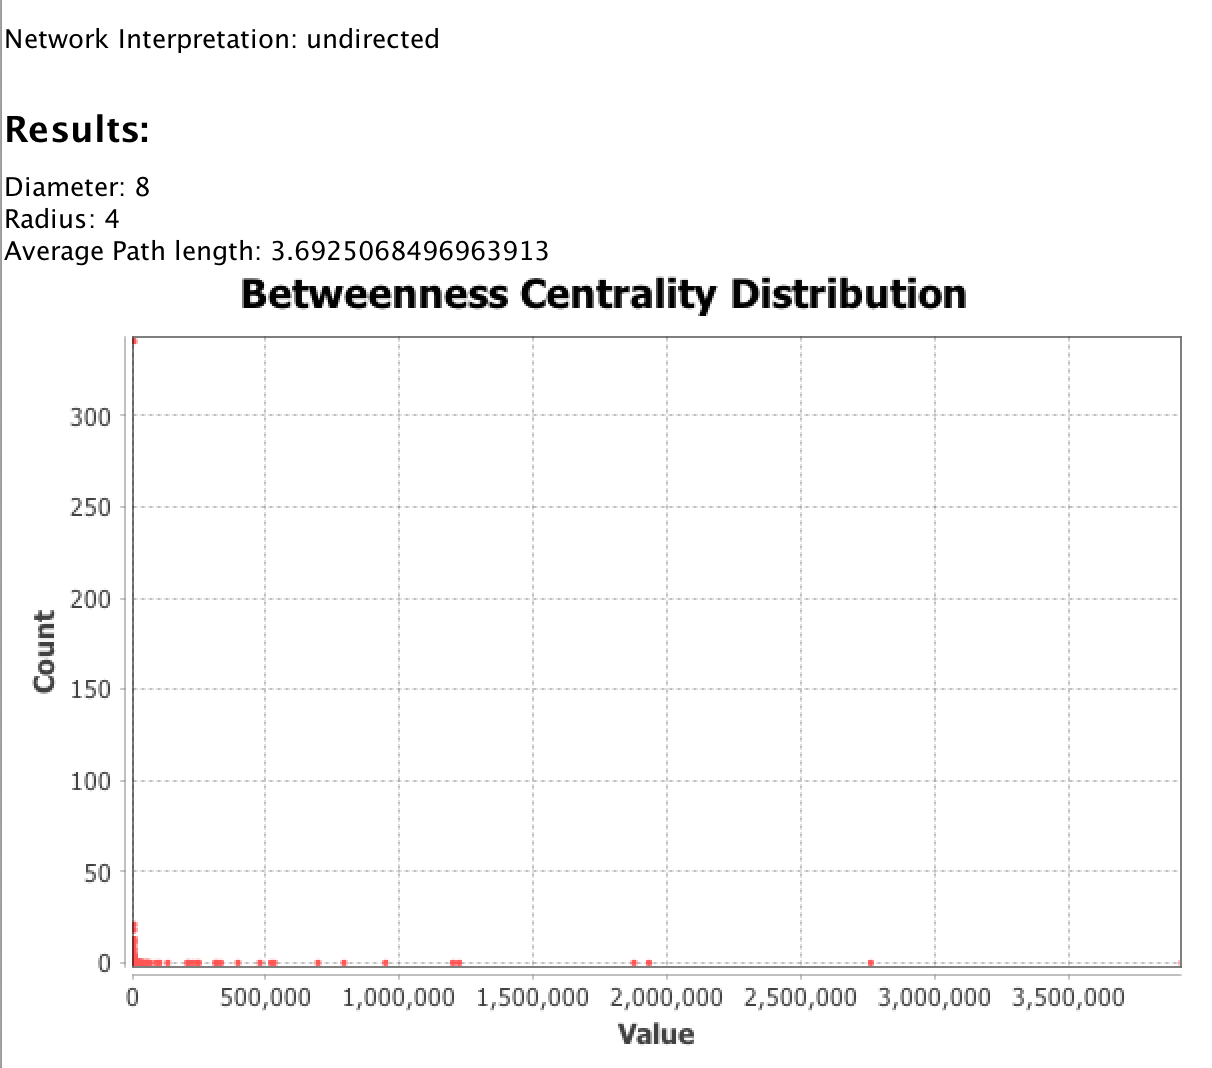
\includegraphics[scale=.2]{BCD.png}
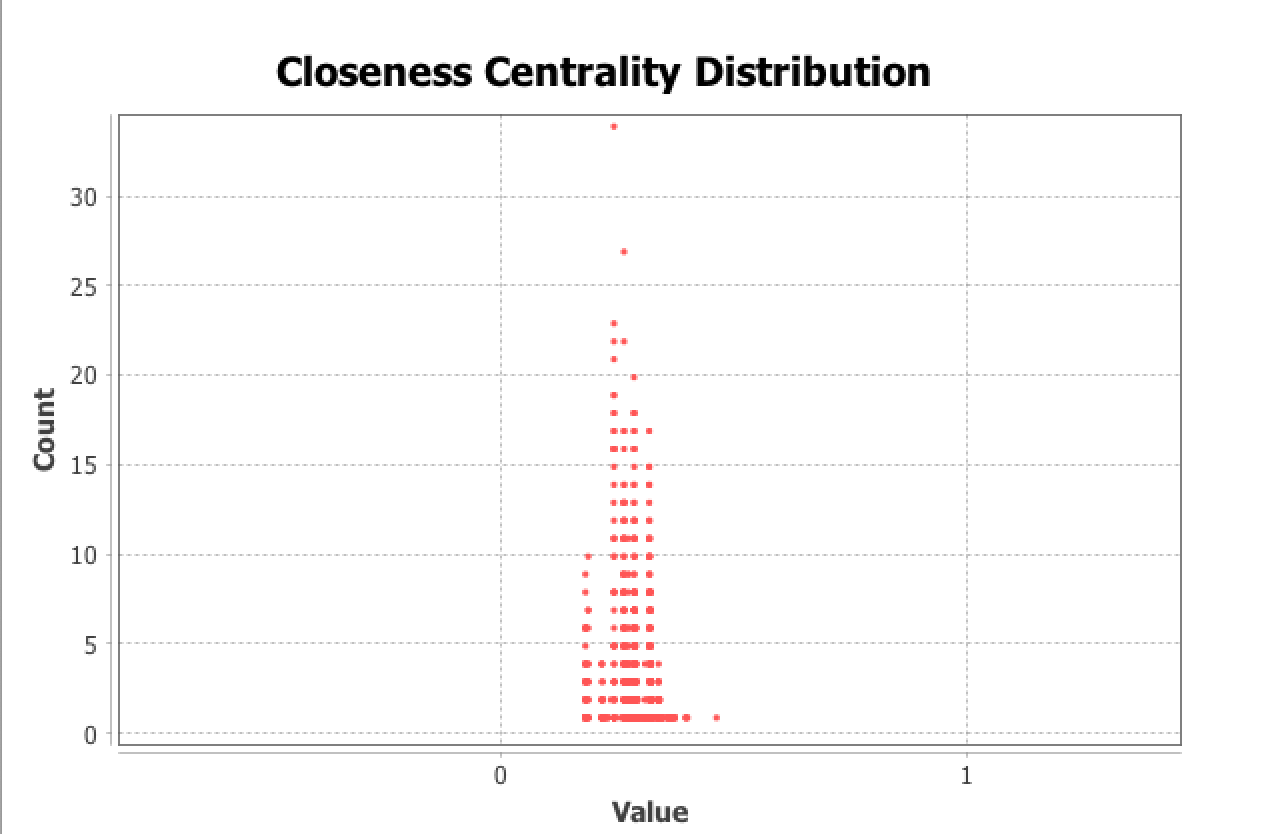
\includegraphics[scale=.2]{CCD.png}
\end{center}


\section{Conclusion}
En conclusión, se obtuvo una buena representación de un tipo de grafo además de extenderlo y exportarlo a más tipos de grafos para así visualizar las semejanzas y diferencias del uso de cada uno. En último término solo se llego a usar la visualización de un archivo solo, en específico el de GraphML, usando la herramienta  Gephi.

\bibliographystyle{plain}
\bibliography{references}
\bibitem{c2} Gephi 2008-2017. GDF Format. Consultado: 30 de octubre de 2019 de https://gephi.org/users/supported-graph-formats/gdf-format/
\bibitem{c3} Gephi. GEXF File Format. Consultado: 30 de octubre de 2019 de https://gephi.org/gexf/format/

\begin{lstlisting}
#include <iostream>
#include <fstream>
#include "Snap.h"
#include <ctime>

typedef PNGraph MyGraphType;

void GraphML(MyGraphType g) {
    std::ofstream file ("fb.graphml");
	if (file.is_open()) {
		file << "<?xml version=\"1.0\"encoding=\"UTF-8\"?>\n";
		file << "<graphml xmlns=\"http://graphml.graphdrawing.org/xmlns\" xmlns:xsi=\"http://www.w3.org/2001/XMLSchema-instance\" xsi:schemaLocation=\"http://graphml.graphdrawing.org/xmlns http://graphml.graphdrawing.org/xmlns/1.0/graphml.xsd\">\n";
		file << "<graph id=\"G\" edgedefault=\"directed\">\n";

		for (MyGraphType::TObj::TNodeI NI = g->BegNI(); NI < g->EndNI(); NI++)
			file << "<node id=\"" << NI.GetId() << "\"/>\n";

		int i = 1;
		for (MyGraphType::TObj::TEdgeI EI = g->BegEI(); EI < g->EndEI(); EI++, ++i)
			file << "<edge id=\"e" << i << "\" source=\"" << EI.GetSrcNId() << "\" target=\"" << EI.GetDstNId() << "\"/>\n";

		file << "</graph>\n";
		file << "</graphml>\n";
		file.close();
	}
}

void GEXF(MyGraphType g) {
	std::ofstream file ("fb.gexf");
	if (file.is_open()) {
		file << "<?xml version=\"1.0\" encoding=\"UTF-8\"?>\n";
		file << "<gexf xmlns=\"http://www.gexf.net/1.2draft\" version=\"1.2\">\n";
		file << "<graph mode=\"static\" defaultedgetype=\"directed\">\n";
		
		file << "<nodes>\n";
		for (MyGraphType::TObj::TNodeI NI = g->BegNI(); NI < g->EndNI(); NI++)
			file << "<node id=\"" << NI.GetId() << "\" />\n";
		file << "</nodes>\n";

		file << "<edges>\n";
		int i = 1;
		for (MyGraphType::TObj::TEdgeI EI = g->BegEI(); EI < g->EndEI(); EI++, ++i)
			file << "<edge id=\"" << i << "\" source=\"" << EI.GetSrcNId() << "\" target=\"" << EI.GetDstNId() << "\" />\n";
		file << "</edges>\n";

		file << "</graph>\n";
		file << "</gexf>\n";
		file.close();
	}
}

void GDF(MyGraphType g) {
	std::ofstream file ("fb.gdf");
	if (file.is_open()) {
		file << "nodedef>id VARCHAR\n";
		for (MyGraphType::TObj::TNodeI NI = g->BegNI(); NI < g->EndNI(); NI++)
			file << NI.GetId() << "\n";

		file << "edgedef>source VARCHAR, destination VARCHAR\n"; 
		for (MyGraphType::TObj::TEdgeI EI = g->BegEI(); EI < g->EndEI(); EI++)
			file << EI.GetSrcNId() << ", " << EI.GetDstNId() << "\n";

		file.close();
	}
}

void JSON(MyGraphType g) {
	std::ofstream file ("fb.json");
	if (file.is_open()) {
		file << "{ \"graph\": {\n";
		file << "\"nodes\": [\n";
		for (MyGraphType::TObj::TNodeI NI = g->BegNI(); NI < g->EndNI(); ) {
			file << "{ \"id\": \"" << NI.GetId() << "\" }";
			if (NI++ == g->EndNI())
				file << " ],\n";
			else
				file << ",\n";
		}

		file << "\"edges\": [\n";
		for (MyGraphType::TObj::TEdgeI EI = g->BegEI(); EI < g->EndEI(); ) {
			file << "{ \"source\": \"" << EI.GetSrcNId() << "\", \"target\": \"" << EI.GetDstNId() << "\" }";
			if (EI++ == g->EndEI())
				file << " ]\n";
			else
				file << ",\n";
		}
		file << "} }";

		file.close();
	}
}

int main() {
	MyGraphType dg = TSnap::LoadEdgeList<MyGraphType>("fb.txt",0,1);
	
	GraphML(dg);

	GEXF(dg);

	GDF(dg);

	JSON(dg);
	return 0;
}
\end{lstlisting}

\end{document}
